\chapter{Design and Methodology}
\label{cha:design-and-method}

Based on our analysis and the information we want to collect, we decided on the following architecture for our system:

\begin{figure}[h]
\centering
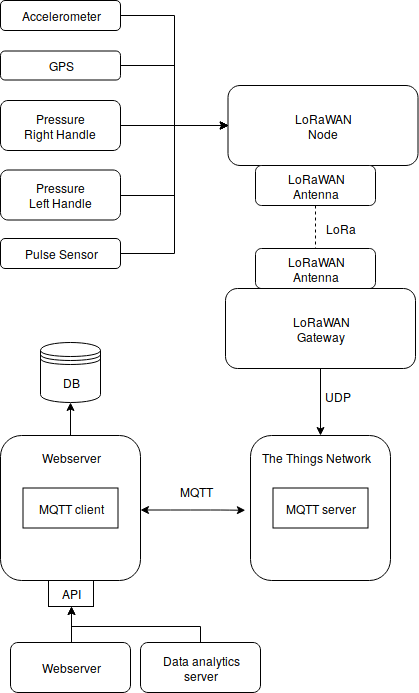
\includegraphics[width=1\linewidth]{gfx/architecture_design_and_methology_h}
\caption{Proposed architecture}
\label{fig:image1}
\end{figure}

\section{Components and their interactions}


	\subsection{LoRaWAN node}
		Polls the sensors in predefined intervals and sends them through LoRaWAN every few minutes

	\subsection{LoRaWAN gateway}
		Receives LoRaWAN packets and relays them to "The Things Network" through the Semtech UDP protocol

	\subsection{The Things Network (TTN)}
		It is possible to have our gateway communicate directly with our server, but we decided to use TTN because it provides some very useful features out of the box, some of them being:

		\begin{itemize}
			\item Node authentication
			\item Packet deserialization
			\item Integration with MQTT, HTTP, Google Cloud, Amazon AWS and Azure
			\item Encryption
			\item Has thousands of registered gateways
		\end{itemize}

		TTN has become the standard in LoRaWAN applications, due to its unparalleled potencial for scalability, integration and security. In our case it deserializes the packets coming from the gateways and publishes them in an MQTT broker 

	\subsection{Server}
		The server will subscribe to the MQTT broker on TTN and store the information received from there, while also exposing an API that can be used, for example, to have other services process the data and display it to the interested parties

% \section{Hardware Decisions}

% 	The proposed architecture can be realized in a number of ways, meaning we had to make the following choices:
% 	\begin{itemize}
% 		\item Use sensors with inbuilt LoRa functionality or use a single-board computer connected to sensors and LoRa transmitter?
% 		\item What hardware to use to interface with the sensors and act as the node?
% 		\item What hardware to use as LoRaWAN gateway?
% 	\end{itemize}


% 	\subsection{Single-board Computer vs Inbuilt LoRa Sensors:}

% 		We had the option of using a single-board computer (SBC) to interface with all of the sensors (Arduino or Rpi) or using sensors with inbuilt LoRaWAN capabilities.

% 		We summarized the haracteristics of sensors with inbuilt LoRaWAN as follows:
% 		\begin{itemize}
% 			\item They require little to no configuration and work out of the box. This means using them would grant us more time to we can focus on other parts of the project.
% 			\item Data can be sent at different rates for each sensor.
% 			\item They are much more expensive than standard sensors.
% 			\item They are bulkier than standard sensors, making them harder to fit into the walker.
% 			\item Their is low variety when it comes to such sensors in the market, limiting choice of vendor and sensors.
% 			\item Having several LoRaWAN transmitters instead of one would make the power consumption higher.
% 			\item Each sensor usually has its own battery or charging method, which makes recharging more complex
% 		\end{itemize}


% 		We summarized the following characteristics of SBCs:
% 		\begin{itemize}
% 			\item Fine grained control of the sensors
% 			\item We might want to do some preprocessing of the sensor data before sending it, which is possible with SBCs.
% 			\item Good amount of variety in the market allowing us a lot of choice.
% 		\end{itemize}

% 		We decided to go with an SBC because we value the flexibility provided by the vast array of sensors to choose from and the possibility to manually program them.



% \subsection{Comparing Raspberry Pi and Arduino:}

% 	We then had the option of either using a Raspberry Pi or an Arduino. We summarized their characteristics as follows:

% 	Pi:
% 	\begin{itemize}
% 		\item Faster and more powerful processor
% 		\item Overhead of operating system, hdmi output, wifi/ethernet port, audio output, all of which take physical or disk space.
% 		\item More power consumption
% 	\end{itemize}

% 	Arduino:
% 	\begin{itemize}
% 		\item Easy to get up and running
% 		\item Easier to connect with analog sensors
% 		\item Lots of different models to choose from, meaning we can choose the one that best fits our goals
% 		\item Cheaper than the Raspberry Pi
% 		\item Smaller 
% 		\item No operating system, meaning we are closer to the hardware and have more control over the sensors
% 	\end{itemize}

% 	Due to the points mentioned above, especially due to its flexibility, and low power consumption, we decided to go with the arduino as the node.

% 	Due to its superior computational power, inbuilt networking capabilities, we decided to go with the Raspberry Pi as the gateway.

% 	Our reasoning is supported by the arguments put forward in \cite{postolache2011smart}.



\section{Experiments}
In order to test the previously mentioned quality parameters and thus our hypothesis, we designed the following experiments:

	\subsection{Normal Usage}
		In order to test the consistency and accuracy of our readings, the reliability of the whole system, its latency, and its energy consumption when in use, we have to use the walker and analyse what output we get. We will thus do two runs of 30 minutes, doing as much as possible to keep all the factors constant and save all the information we get. We can then use the sensor readings to find out our consistency and accuracy, the percentage of packets dropped for latency, the delay between them for latency and the energy used for energy consumption.

	\subsection{Idle Energy Consumption}
		We will leave the walker idle for around 12 hours while measuring its energy comsumption.
		We can then calculate how much energy the node consumes per hour both idle and in use (above experiment) and conclude how much it will last on common 9V batteries.

	\subsection{Integrating the GPS sensor}
		In order to test the modularity of the system, we will deliberately only integrate the GPS sensor in the testing phase of the project, this way we can measure how much time it takes and analyse the complications brought by doing so.

	\subsection{Setting up the Arduino from scratch}
		Due to the fact that we only have one LoRaWAN hat for the Arduino, we are not able to have two setups running simultaneously, so we will re-register the arduino in "The Things Network" and re-upload the code to it, measuring how much time the process takes. We will do it once without practicing the process, and then one more time when we know exacly which steps to take. This experiment is the closest we can get to testing the scalability of our system.

	\subsection{Disconnecting cables}
		In order to test serviceability, we will have someone disconnect random cables connecting the sensors to the node and we will then have another member of the team get the system back up and running while we measure the time it takes.

	\subsection{Finding maximimum throughput}
		We will increase the ammount of bytes being sent by the node until they no longer arrive, this will allow us to discover the maximum amount of information we are able to send in each packet.





% \subsection{Consistency}
% To test consistency we will devise some usage scenarios and for each of them get 10 measurements. We will then compare the precision within and between scenarios by getting the variance.

% \subsection{Accuracy}
% In order to measure accuracy we need to find the difference between the measured value of each sensor and compare it to the true value. This means we need a test tailored to each sensor. For this, we will perform 10 measurements from each sensor and then find the standard deviation of the measured values from the true value.

% \subsection{Reliability}
% To measure reliability we will use the walker for 30 minutes and calculate the percentage of times the sensor data got stored in the server’s database

%%% Local Variables:
%%% mode: latex
%%% TeX-master: "../ClassicThesis"
%%% End:
